%-------------------------------------------------------------------------------
% seq66 sessions
%-------------------------------------------------------------------------------
%
% \file        sessions.tex
% \library     Documents
% \author      Chris Ahlstrom
% \date        2020-10-03
% \update      2020-11-21
% \version     $Revision$
% \license     $XPC_GPL_LICENSE$
%
%  Provides a discussion of how Seq66 supports session management, specifically
%  the Non Session Manager.
%
%-------------------------------------------------------------------------------

\section{Seq66 Session Management}
\label{sec:sessions}

   The first thing to do for session management is to make sure that the
   application is capable of various levels of session management, from
   \textsl{UNIX} signals to
   a complete session manager like the \textsl{Non Session Manager}.
   Basic session management consist of being able to properly start the
   application and let it run properly during its life-cyle, whether it is a
   command-line application or a graphical application.

   \textsl{Seq66} supports session management in three ways:

   \begin{enumber}
      \item \textbf{Non Session Manager} (NSM)
      \item \textbf{Signals}
      \item \textbf{LASH} (not ready)
   \end{enumber}

   \textbf{Non Session Manager} provides a replacement for the
   \textsl{JACK Session API} (now disabled by default in a \textsl{Seq66}
   build).  It allows control over the startup of multiple applications, the
   process of saving a session, and
   provides a way to save their patching (connections) in \textsl{JACK}.
   \textsl{NSM} support in \textsl{Seq66} is essentially finished.

   \textbf{Signals} provide for initiating a save operation and the sudden
   termination of an application.  This mode is useful with
   \textsl{nsm-proxy}, a way to script applications that don't have \textsl{NSM}
   support.

   \textbf{LASH} is an earlier session protocol, supported in \textsl{Seq64}.
   However, it is not ready in \textsl{Seq66} and is a low priority at this time.

%  See \sectionref{subsec:rc_file_midi_control},

\subsection{Seq66 Session Management / NSM}
\label{subsec:sessions_nsm}

   \index{sessions!nsm}
   The \textsl{Non Session Manager} is an API implementation for session
   management for Linux audio/MIDI. NSM clients use a well-defined
   \index{sessions!OSC}
   \textsl{OSC} protocol to communicate with the session management daemon.

\subsubsection{Seq66 Session Management / NSM / First Run Without NSM}
\label{subsec:sessions_nsm_first_run_without_nsm}

   This section discusses what happen when \textsl{Seq66} is installed, then
   run outside of any session from the console or an application menu.
   For a discussion where \textsl{Seq66} is run for the first time under
   \textsl{NSM},
   see \sectionref{subsec:sessions_nsm_first_run_in_nsm}.

   Generally, after installing \textsl{Seq66}, or when creating a new setup
   (such as a playlist) it is good to run it normally first, to simplify
   trouble-shooting.
   This action creates the configuration files in the default location,
   \texttt{/home/user/.config/seq66}:

\begin{verbatim}
   $ qseq66 
   [No 'rc' file, will create: qseq66.rc/ctrl/midi/mutes]
   [No 'usr' file, will create: /home/user/.config/seq66/qseq66.usr]
   [File exists: /home/user/.config/seq66/qseq66.rc]
   [Saving initial config files to session directory!]
   [Writing 'rc': /home/user/.config/seq66/qseq66.rc]
   [Writing 'ctrl': /home/user/.config/seq66/qseq66.ctrl]
   [Writing 'mutes': /home/user/.config/seq66/qseq66.mutes]
   [Writing 'usr': /home/user/.config/seq66/qseq66.usr]
   . . .
\end{verbatim}

   Then exit \textsl{Seq66} to ensure the configuration files are created.
   Optionally, in this initial setup,
   one can also create a 'playlist' file and a 'drums' file, or
   copy them from \texttt{/usr/share/seq66-0.91/data/samples} to
   \texttt{/home/user/.config/seq66} and modify them appropriately.
%  Generally, it is best to make sure that \texttt{qseq66} runs normally before
%  attempt to get it work in a session.

   Another first-time modification to consider is setting up \textsl{Seq66} to
   use the \textsl{JACK} audio/MIDI subsystem (on \textsl{Linux}).
   In the 'rc' file, look for the following line:

\begin{verbatim}
   0   # with_jack_midi
\end{verbatim}

   And change it to:

\begin{verbatim}
   1   # with_jack_midi
\end{verbatim}

   Another first-time modification to consider is using virtual ports (option
   \texttt{--manual-ports}) versus the automatic port connections
   \textsl{Seq66} normally makes.
   This setup allows the user to manually make connections between
   \textsl{Seq66} and other MIDI applications.
   In the 'rc' file, look for the following lines:

\begin{verbatim}
   [manual-ports]
   0   # flag for manual (virtual) ALSA or JACK ports
   16  # number of manual/virtual ports
\end{verbatim}

   And change them to:

\begin{verbatim}
   [manual-ports]
   1   # flag for manual (virtual) ALSA or JACK ports
   4   # number of manual/virtual ports
\end{verbatim}

   It is then important to start \texttt{qseq66} in the normal manner again,
   and verify that everything works as expected.

\subsubsection{Seq66 Session Management / NSM / Run in NSM}
\label{subsec:sessions_nsm_first_run_in_nsm}

   When \textsl{Seq66} is run in \textsl{NSM} for the first time,
   what happens to the new configuration depends on whether or not 
   the normal configuration files exist in the default location,
   \texttt{/home/user/.config/seq66}.

   If these normal configuration files exist, then they are replicated in the
   \textsl{NSM} session directory.  If a playlist has been configured, it is also
   copied, and so are the MIDI files it requires. (Their relative directory
   structure is preserved.)
   If these files do not exist, then new configuration files are created
   in the \textsl{NSM} session directory.

   \textbf{No existing normal configuration}.
   Here, we have just installed \textsl{Seq66}, but have not
   yet run it.  We start the \textsl{non-session-manager}, create a new session,
   and add \texttt{qseq66} to this session.  This starts \texttt{qseq66}, and,
   after a short delay to get the session information from the daemon, a new
   configuration is created in the session directory.

   \textbf{Existing normal configuration}.
   If there is an existing \textsl{Seq66} configuration (in
   \texttt{/home/user/.config/seq66}, then running \texttt{qseq66} in a new
   session will cause the configuration to be recreated in the new session
   directory, including play-lists and MIDI files.

   If \textsl{JACK} has been configured to be
   used by \textsl{Seq66}, be sure \textsl{JACK} is started (e.g. by running
   the \textsl{qjackctl} application.)

   For illustration, we run \textsl{NSM} from a terminal window, which can be
   very helpful when problems occur.

\begin{verbatim}
   $ non-session-manager
   [non-session-manager] Starting daemon...
   [nsmd] Session root is: /home/user/NSM Sessions
   NSM_URL=osc.udp://mycomputer.mls:19625/
   [nsmd] Listing sessions
\end{verbatim}

   \index{sessions!non-starter}
   If \textsl{NSM} refuses to start, make sure that the \texttt{liblo} library
   from the OSC project is installed.  If it is installed, then check the
   \texttt{/etc/hosts} file to make sure that the loopback interfaces are
   defined. In some versions of \textsl{Linux}, it isn't defined properly,
   and the \textsl{NSM} daemon (\texttt{nsmd}) will not start.
   Here is an example for the default install in \textsl{Debian Sid};

\begin{verbatim}
   127.0.0.1   localhost
   127.0.1.1   mycomputer.mls mycomputer
\end{verbatim}

   The NSM user-interface (not shown here) that comes up is empty at first.  So
   we create a session by clicking the \textsl{NSM}
   \textsl{New} button, and entering a session name (e.g. "Seq66") in the
   prompt that comes up.  We see, in the console window, a couple of 
   \texttt{/nsm/server/new} \textsl{OSC} messages
   about the creation of the session.

\begin{verbatim}
   [non-session-manager] Sending new for: Seq66
   [nsmd] Creating new session "Seq66"
   [non-session-manager] /nsm/server/new says Created.
   [non-session-manager] /nsm/server/new says Session created
\end{verbatim}

   Next, we click the \textsl{Add Client to Session}, and, since
   \texttt{qseq66} has been installed, it is in the \texttt{PATH}
   and its executable name can be entered simply: "qseq66".
   A number of console messages from
   \textsl{Seq66} appear, plus some messages from \textsl{NSM}.

\begin{verbatim}
	[non-session-manager] Sending add for: qseq66
	[nsmd] Process has pid: 2797436
	[nsmd] Launching qseq66
	[nsmd] Got announce from seq66
	[nsmd] Client was expected.
	[nsmd] Process has pid: 2797436
	[nsmd] The client "seq66" at "osc.udp://127.0.0.1:13318/" informs us it's
    ready to receive commands.
\end{verbatim}

	Once \textsl{Seq66} is running under \textsl{NSM},
   then click the "Save" button at the top of the \textsl{NSM} interface in order
   to save the session information.  This is an important step.
   We can see what has been created to support the session.
   The directory that \textsl{NSM}
   creates by default is \texttt{/home/user/NSM Sessions}.

\begin{verbatim}
   $ pwd
   /home/user/NSM Sessions
   $ lstree Seq66
	Seq66/
	  +-- seq66.nGJDW/
	  |   +-- config/
	  |   |   +-- qseq66.ctrl
	  |   |   +-- qseq66.mutes
	  |   |   +-- qseq66.rc
	  |   |   +-- qseq66.usr
	  |   +-- midi/
	  +-- session.nsm
\end{verbatim}

	So \textsl{NSM} has created a directory with the session name we gave it:
   \texttt{Seq66}.  Under that directory is a file, \texttt{session.nsm}, which
   contains information like the following when we click the \textsl{Save}
   button at the top of the \textsl{NSM} user-interface:

\begin{verbatim}
   seq66:qseq66:nIRJI
\end{verbatim}

   The format of this text is \texttt{appname:exename:nXXXX}.
   Also created is a directory, \texttt{seq66.nIRJI}, which is the root of the
   \texttt{Seq66} session.  The "IRJI" portion is randomly generated by
   \textsl{NSM}.

   The rest of the directories are generated by \textsl{Seq66}, which creates
   new \texttt{config} directory (to be used instead of
   \texttt{/home/user/.config/seq66}) and a \texttt{midi} directory which will
   contain any new, imported MIDI files, or MIDI files from the playlist.
   The new \texttt{config} directory
   contains versions of the various configuration files that will always be
   used to start up \textsl{Seq66} during the session.
   One can also add valid play-list and drums/note-mapping files to that
   directory later.

   Note that, if before running \textsl{NSM},
   one had set up a playlist file and provided the proper "MIDI
   base directory" in the 'rc' file, then all the MIDI files will be copied to
   the \textsl{NSM} session directory.
   When the \textsl{Non Session Manager} is started the next time, and the
   "Seq66" session is clicked, this starts \textsl{Seq66}, and the playlist can
   be seen in the \textsl{Playlist} tab.

   One last thing to note is that, when viewing the MIDI ports created by
   \textsl{Seq66}, they will be named "seq66" when not in session management,
   and "seq66.nIRJI" (for example) when under session management.  This makes
   it possible to run multiple instances of \textsl{Seq66}.

\subsubsection{Seq66 Session Management / NSM / Run with Remote NSM}
\label{subsec:sessions_nsm_before_using_nsm}

   As described in the \textsl{NSM} documentation, the \texttt{nsmd} daemon can
   be run stand-alone, and can also be ran on a remote computer.
   The \texttt{qseq66.usr} file can be edited to allow \textsl{Seq66} to
   use a pre-planned \textsl{NSM} and specify the URL to connect.
   Look for the following lines in the 'usr' file:

\begin{verbatim}
   [user-session]
   session = none
   url = ""
\end{verbatim}

   Now assume we've run the daemon as follows:

\begin{verbatim}
   $ nsmd --osc-port 9999
   [nsmd] Session root is: /home/user/NSM Sessions
   NSM_URL=osc.udp://mycomputer.mls:9999/
\end{verbatim}

   Change the \texttt{session} lines to allow the usage of
   \textsl{NSM} at that URL:

\begin{verbatim}
   [user-session]
   session = nsm
   url = "osc.udp://mycomputer.mls:9999"
\end{verbatim}

   The \texttt{url} is not used if running \textsl{Seq66} from the \textsl{NSM}
   GUI... the application will get the URL from the \textsl{NSM} environment.

   Note that \texttt{qseq66} can still be run outside of a
   session manager.  It will detect the absense of the session manager and run
   normally.

\subsubsection{Seq66 Session Management / Sessions Tab}
\label{subsubsec:sessions_tab}

   The \textsl{Session} tab is provided to orient the
   user to the setup supported by the session.
   When not running in a session, the normal configuration directory and files
   are shown.  When running in an \textsl{NSM} section, the configuration
   information received from \textsl{NSM} is displayed.

   This tab is not yet fully functional and is meant to display information to
   help the user understand what is happening in the run.  In particular, the
   \textbf{Detach} and \textbf{Session Log} don't yet work.

\begin{figure}[H]
   \centering 
   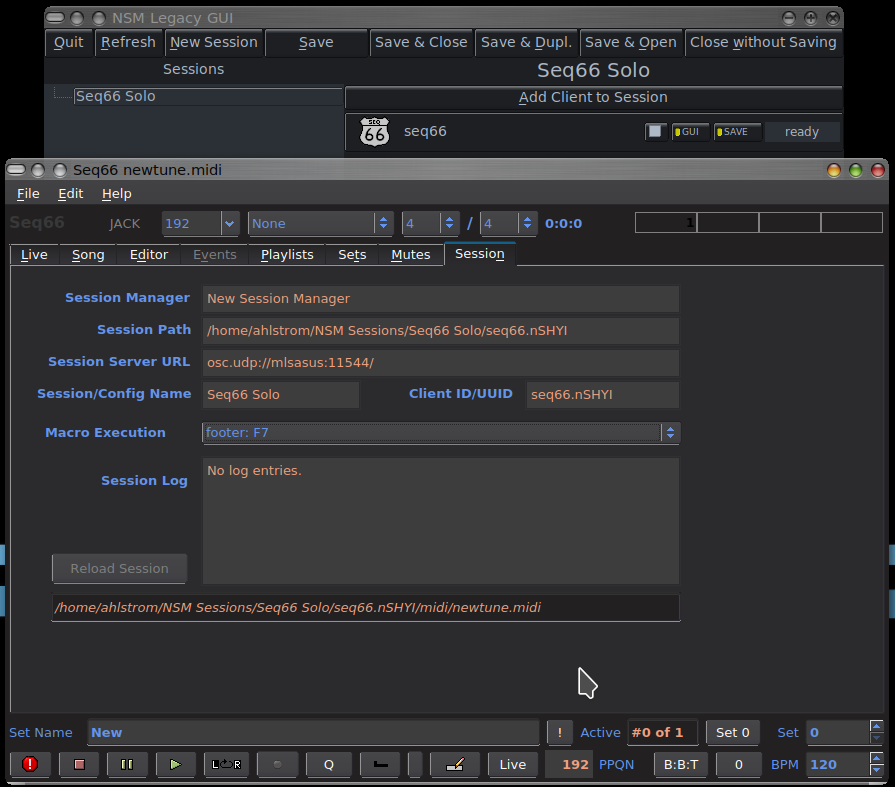
\includegraphics[scale=0.65]{tabs/session/qseq66-session-tab.png}
   \caption*{Session Tab When Running Under NSM}
\end{figure}

   \index{sessions!ui}
   This section describes the \textsl{Session} tab in the main
   \textsl{Seq66} window.  At present, this tab is just informative.  It
   displays the following bits of information that \textsl{Seq66} has received
   from \textsl{NSM} via the \texttt{nmsd} daemon:

   \begin{itemize}
      \item Name of the session manager.
      \item Session path for the session, the root directory of the session.
         All data goes into this directory. If not running in a session,
         the active configuration directory (which can be changed via the
         command-line arguments) is shown.
      \item The OSC URL of the session, which includes the port number.
         Generally, the port number is selected at run-time, but it is also
         possible to configure \textsl{NSM} to use a specific port number.
      \item Display-name for the session.
      \item The generated client ID for the session.
      \item The log of action of the session manager. Not yet supported.
   \end{itemize}

\subsubsection{Seq66 Session Management / File Menu}
\label{subsubsec:sessions_file_menu}

   The author of \textsl{NSM} has provided documentation for session-management
   which provides very strict instructions on how an application must behave
   under session management.  \textsl{Seq66} tries very hard to stick to these
   instructions.  One major adjustment an application must make is to adhere to
   the "File menu" guidelines.

\begin{figure}[H]
   \centering 
   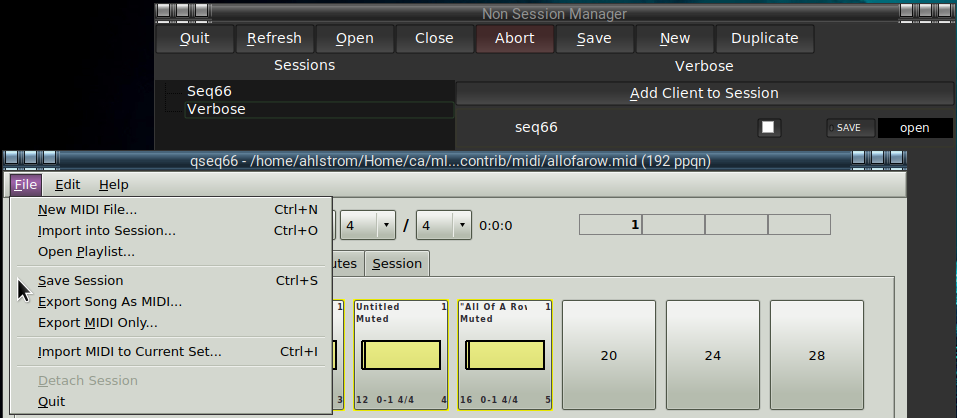
\includegraphics[scale=0.65]{tabs/session/nsm-qseq66-menus.png}
   \caption*{File Menu When Running Under NSM}
\end{figure}

   The following items describe the menu entries.  Some of these may be in
   progress or still need to be enforced.

   \begin{itemize}
      \item \textbf{New MIDI File}.
         This function prompts for the name of a
         new MIDI file and clears the current MIDI file.  The file-name must not
         include a full-path to the file.  The path is hardwired by the
         session.  A relative path can be included.  This name is needed
         because there is no "Save As" option when running in an \textsl{NSM}
         session.
      \item \textbf{Import into Session}.
         Prompts the user for a MIDI file to
         be imported (copied) into the current session.  The path to the file
         is then adjusted to use the \textsl{NSM} \texttt{midi} subdirectory.
      \item \textbf{Open Playlist}.
         Works the same as without session
         management, but gets the list from the session directory.
      \item \textbf{Save Session}.
         This function saves the main configuration
         files (except for the 'usr' file), saves the play-list and note-mapper
         files, if in use, and saves the current MIDI file, if any.
      \item \textbf{Export Song As MIDI}.
         Allows exporting the current song as a stock MIDI file, using the
         performance information (triggers) to write the MIDI data as it would
         be played in "song" mode.
         The default directory that comes up in the
         prompt is the "last-used directory" from the session 'rc' file.
      \item \textbf{Export MIDI Only}.
         Allows exporting the current song as a stock MIDI file.
         The "proprietary" SeqSpec data is \textsl{not} written.
         The default directory that comes up in the
         prompt is the "last-used directory" from the session 'rc' file.
      \item \textbf{Import MIDI to Current Set}.
         This item allows the user to grab a MIDI file from anywhere and import
         it into the current set.
         The default directory that comes up in the
         prompt is the "last-used directory" from the session 'rc' file.
      \item \textbf{Detach}.
         Allows \textsl{Seq66} to detach from session management.
         This process simply disconnects from \textsl{NSM} and restores the
         normal \textsl{File} menu.
         Currently, it is disabled because it causes issues that we cannot yet
         solve.
      \item \textbf{Quit}.
         Quits \textsl{Seq66}.
         There are no messages to send to \textsl{NSM} in this case.
         The \texttt{nsmd} daemon detects that the \textsl{Seq66} client has
         disappeared (and notes that on the console output, if available).
   \end{itemize}

\subsection{Seq66 Session Management / Signals}
\label{subsec:sessions_signals}

   \index{sessions!signals}
   By default, the basic form of session management in
   \textsl{Seq66} occurs by signals.  A
   session manager can start \textsl{Seq66}, and it can tell \textsl{Seq66} to
   save or stop.  Starting is done by a system call to spawn the application.
   The save and stop actions are supported by sending the following signals to
   the application:

   \begin{itemize}
      \item \texttt{SIGINT}.
         This signal stops \textsl{Seq66}. It corresponds
         to using \texttt{Ctrl-C} from the command-line to stop \textsl{Seq66}.
         This signal should work for both the graphical and command-line
         application.  As \textsl{Seq66} shuts down, it does its normal saving
         of the current state of the configuration.
      \item \texttt{SIGTERM}.
         This signal also stops \textsl{Seq66}.  It can
         be sent by an application to exit \textsl{Seq66}.
      \item \texttt{SIGUSR1}.
         This signal tells \textsl{Seq66} to save.  This
         action will save the current MIDI file.
   \end{itemize}

   One application that can control \textsl{Seq66}, to some extent, when not in
   session mode, is \textsl{nsm-proxy}:

      \url{https://non.tuxfamily.org/wiki/nsm-proxy}

   \textsl{NSM-Proxy} is a simple \textsl{NSM} client for wrapping non-NSM
   capable programs. It enables the use of programs supporting LADISH Level 0
   and 1, and programs which accept their configuration via command-line
   arguments.  There is a command-line version and a graphical version.

   MORE TO COME on how to use nsm-proxy.

\subsection{Seq66 Session Management / LASH}
\label{subsec:sessions_lash}

   \index{sessions!lash}
   MORE TO COME.
   LASH support has not yet been fully reimplemented and retested.

%-------------------------------------------------------------------------------
% vim: ts=3 sw=3 et ft=tex
%-------------------------------------------------------------------------------
